\documentclass[dvipdfmx,uplatex]{jsarticle}

%% Packages
\usepackage{graphicx,color,hyperref}
\usepackage{algorithm}
\usepackage{algorithmic}
\usepackage{url}
\usepackage{lscape}
\usepackage{mathtools}
\usepackage{here}
\usepackage{amsmath,amssymb,amsfonts}
\usepackage{amsthm}
\usepackage{tikz}
\usepackage{tcolorbox}
\usepackage{pxjahyper}

%% Theorem Styles
\newtheorem{theorem}{定理}
\newtheorem{proposition}{命題}
\newtheorem{cor}{系}
\newtheorem{definition}{定義}
\newtheorem{problem}{問題}
\theoremstyle{remark}
\newtheorem{remark}{注意}
\newtheorem{requirement}{条件}

%% Environment (Colorful Box)
\newenvironment{simplebox}{
    \begin{tcolorbox}[
        fonttitle=\bfseries,
    ]
}{
    \end{tcolorbox}
}

\newenvironment{method}[1]{
    \begin{tcolorbox}[
        colframe=green!50!black,
        colback=green!50!black!10!white,
        colbacktitle=green!50!black!40!white,
        coltitle=black,
        fonttitle=\bfseries,
        title={#1}
    ]
}{
    \end{tcolorbox}
}

\newenvironment{experiment}[1]{
    \begin{tcolorbox}[
        colframe=violet,
        colback=violet!10!white,
        colbacktitle=violet!40!white,
        coltitle=black,
        fonttitle=\bfseries,
        title={#1}
    ]
}{
    \end{tcolorbox}
}

\newenvironment{kansou}{
    \begin{tcolorbox}[
        colframe=brown,
        colback=brown!10!white,
        colbacktitle=brown!40!white,
        coltitle=black,fonttitle=\bfseries
    ]
}{
    \end{tcolorbox}
}

%% Title
\title{Sphinteract: Resolving Ambiguities in NL2SQL Through User Interaction}
\author{\empty}
\date{\empty}

%% Document body
\begin{document}
\maketitle

\begin{itemize}
    \item Link: \url{https://www.vldb.org/pvldb/vol18/p1145-zhao.pdf}
    \item Conference: VLDB2025
    \item Citation:
    \item Arxiv:
\end{itemize}

\section{概要}
\begin{simplebox}
\begin{itemize}
    \item NL2SQLにおいて、ユーザが発する質問の曖昧性を解消するためのフレームワークSpinteractを提案する。これはあいまいさを解消するためにユーザフィードバックを対話的に取り入れる。
    \item ユーザフィードバックを取り入れるための質問はSummarize, Review, Askという3つの方針のどれかに基づいて生成される(SRAパラダイム)。
    \item SpinteractによってKaggleDBQA、BIRDによる実験で最大で42\%の精度向上が達成できることを示した。
\end{itemize}
\end{simplebox}

\section{問題設定}
\begin{simplebox}
\begin{itemize}
    \item 解答の流れと定式化
    \begin{itemize}
        \item ユーザの自然言語の質問に対して、SQLクエリを生成する。このクエリが誤っている場合は対話プロセスが開始され、ユーザに質問が提示される。ユーザの回答を受け取った後、SQLクエリが修正される。このプロセスは正しいSQLクエリが生成されるか、停止基準が満たされるまで繰り返される。
        \item この条件の下で、ラウンド数$n$とLLM呼び出しのコストに依存するあるコスト関数を最小化するというように定式化される。
    \end{itemize}
    \item 求められる条件として
    \begin{itemize}
        \item ユーザへの質問はSQLがわからない人にとっても理解可能であること
        \item ユーザへの質問への解答は簡単であること: 選択肢方式など
        \item 無限に質問ができるわけではないため、不要なやりとりを避ける必要がある: 固定回数の方式と、あいまいさが検出されなくなった時点で停止する方式の両方を検討する
        \item ユーザに実行可能なクエリが提示できること
    \end{itemize}
\end{itemize}
\end{simplebox}

\section{自然言語の質問に曖昧性があることの検証}
\begin{simplebox}
\begin{itemize}
    \item KaggleDBQAからランダムに64この質問を抽出し、これらの質問に曖昧性があることを検証する。具体的には次のようにした。
    \item 複数人に選んだ質問のSQLを作成してもらい、これらの実行結果がどの程度一致するかを検証した。
    \item その結果64問中8\%しかそれは一致しなかった。また最も可能性の高い回答の割合についても調べたが、およそ50\%の質問しか多数派(50\%を超える)の回答が存在しなかった。
\end{itemize}
上の結果をもとに、あいまい性の種類を分類した。
\begin{itemize}
    \item AmbColumn: 質問内のエンティティがデータスキーマと明確に対応付けられない場合(e.g. 似たカラムが複数存在する、カラムが不明瞭など)
    \item AmbOutput: 出力テーブルの形式や並び順が指定されていない場合
    \item AmbQuestion: 質問が漠然としている場合
    \item AmbValue: 使用すべき述語値に不確実性がある場合に発生する(たとえば数値であるべき値が文字列として与えられた場合など)
\end{itemize}
\end{simplebox}

\begin{figure}
    \centering
    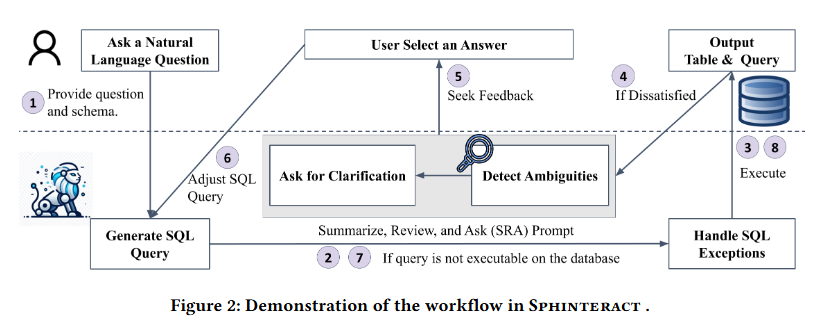
\includegraphics[width=0.5\textwidth]{img/sphinteract/overview.png}
    \caption{Sphinteractの概要}
    \label{fig:overview}
\end{figure}

\section{手法}
\begin{method}{Sphinteract}
\begin{itemize}
    \item Sphinteractフレームワークはユーザとのマルチラウンドの対話で構成される、このプロセスは次の二つの部分に分けられる(1. SQLクエリの生成、2. ユーザとの対話)。図\ref{fig:overview}に示される。
    \begin{itemize}
        \item まず自然言語とデータベーススキーマのみを用いてSQLクエリを生成する。
        \item このクエリを実行し、出力とクエリをユーザに提示する。ユーザはこのクエリが期待に添わない場合に、その旨をフィードバックする。
        \item フィードバックをもとに複数選択式質問を生成し、ユーザに提示してFBを得る。
        \item このSQLクエリと実行結果をユーザに提示する。
        \item このプロセスを終了条件が満たされるまで続ける。
    \end{itemize}
    \item SQL生成はDAIL-SQLのプロンプトを用いる。
    \item CQ: 曖昧性解消のための質問の生成のプロンプトには誤ったクエリとそのFBを入力として使用する。ここではSRA(Summarize, Review, Ask)という新手法を導入する。すなわち、これまでの対話から情報を要約し、残る曖昧性を評価し、あいまい性解消のための質問をユーザに提示する。
    \item ES: すべての曖昧性を除去した場合でもSQLを生成できない場合があり、この場合に無限にこのプロセスが続くことを防ぐために、Early Stoppingができるようにする(曖昧性がない場合には終了できることをプロンプトに書いておく)。
\end{itemize}
\end{method}


\section{実験結果}
\begin{experiment}{実験手法}
\begin{itemize}
    \item 
\end{itemize}
\end{experiment}

\begin{experiment}{実験結果}
\begin{itemize}
    \item Zero Shotの場合
    \begin{itemize}
        \item 
    \end{itemize}
    \item Few Shotの場合
    \begin{itemize}
        \item 
    \end{itemize}
    \item Userスタディ
    \begin{itemize}
        \item 
    \end{itemize}
\end{itemize}
\end{experiment}

\section{感想}
\begin{kansou}
\begin{itemize}
  \item ユーザの質問に曖昧性がある場合にインタラクティブにユーザ意図を確認することでNL2SQLの精度向上を目指していて、現実に近い環境を考慮している点が面白いと思った。
\end{itemize}
\end{kansou}

\begin{figure}
    \centering
    
\includegraphics[width=0.5\textwidth]{img/image.png}
    \caption{キャプション}
    \label{fig:template}
\end{figure}

\bibliographystyle{jplain}
\bibliography{template.bib}

\end{document}